\documentclass[12pt,a4paper]{article}
\usepackage[top=25.4mm, bottom=25.4mm, left=19.1mm, right=19.1mm]{geometry}


\usepackage[latin2]{inputenc}
\usepackage{graphicx}
\graphicspath{ {./images/} }
\usepackage{ulem}
\usepackage{amsmath}
\usepackage[document]{ragged2e}

\setlength{\parindent}{4em}
\setlength{\parskip}{1em}
\usepackage{hyperref}

\usepackage{fancyhdr}
\pagestyle{fancy}
\fancyhf{}
\fancyhead[LO]{\textbf{\small IoT and Smart Analytics}\\
\text{\small A Program by IIITH and TalentSprint}}

\usepackage{xcolor}
\usepackage{lipsum}

\rhead{\begin{picture}(0,0) \put(-250,-2){
\includegraphics[width=9cm]{EXP_08_Images/ts-iisc-logo-pr.png}} \end{picture}}
\cfoot{\thepage}


\begin{document}

\begin{center}

\textbf{\large \\EXPERIMENT 04 }\\[6pt]
Programming Arduino
\end{center}

\textbf{\large LEARNING OBJECTIVES:}\\[3pt]
At the end of this experiment, participants will be able to:\vspace{-6mm}\begin{enumerate}
 \setlength\itemsep{-0.3em}
\item understand the serial monitor \& plotter for printing/reading/plotting data \& related functions.
\item understand strings and character functions
\item understand Math library
\item understand the functions: digitalRead(), analogRead()/analogWrite() \& PWM
\item use variable, loop, conditional statement \& define functions with Arduino
\item implement all above concepts in both TinkerCAD and actual hardware with Arduino

\end{enumerate}
\textbf{\large APPARATUS REQUIRED:}\\
\vspace{-0.1mm}
\begin{enumerate}
\setlength\itemsep{-0.1em}
\item A good internet connection
\item Arduino-1pcs
\item Power adapter-1pcs
\item LED: Red, Green, Blue -1pcs each
\item Resistor 1 k$\Omega$ -3pcs
\item 10 k$\Omega$ Potentiometer-1pcs
\item Push-button -2pcs
\item Breadboard-1pcs
\item Jumper wires
\item Buzzer-1pcs



\end{enumerate}
\begin{justify}
\textbf{\large THEORY}\\[3pt]
\textbf {\underline {Serial Communication}}\\[3pt]
Followings are the few frequently used functions of the Serial class available in Arduino for communicating with computer/other devices. See appendix for detail of following functions.
\begin{center}
\textbf { Serial.begin(speed), Serial.print(),  Serial.println(), Serial.available(), Serial.read(), Serial.readString(), Serial.parseFloat(), Serial.parseInt(), Serial.write()} 
\end{center}
\noindent All the above functions will be used in the following examples in conjunction with other operations and applications. But, we will not design an experiment to show only the above functions explicitly.\\

\vspace{2cm}
\noindent \textbf{\large PROCEDURE}\\[3pt]
\textbf {\underline {Strings}}\\[3pt]
The text enclosed inside double quotes is strings. The \textbf {string} is a data type that stores text rather than integer values. It is similar to other data types such as integer, float, etc., in Arduino. The string is an array of characters consisting of \textbf {numbers, spaces, and special characters} from the ASCII table.
Strings can be declared in different ways. We are going to see few examples below implementing strings in Arduino.\par
\noindent \textbf{Hardware/Software Setup:} Since all these examples are taking input from the serial monitor and printing back to the serial monitor, we don't have to connect any other device except the Arduino board. Connect the Arduino board to the PC, upload the code, and interact with the serial monitor as per the code. The serial monitor is found on the right top corner a tiny graphics showing an image of a lens or inside the Tools menu (fig. 1). Do not forget to set the correct baud rate as given in code, shown in fig. 2 below. In TinkerCAD, drag the Arduino to the workspace, dump the code, and interact with the serial monitor provided there.
\vspace{-3mm}
\begin{center} 
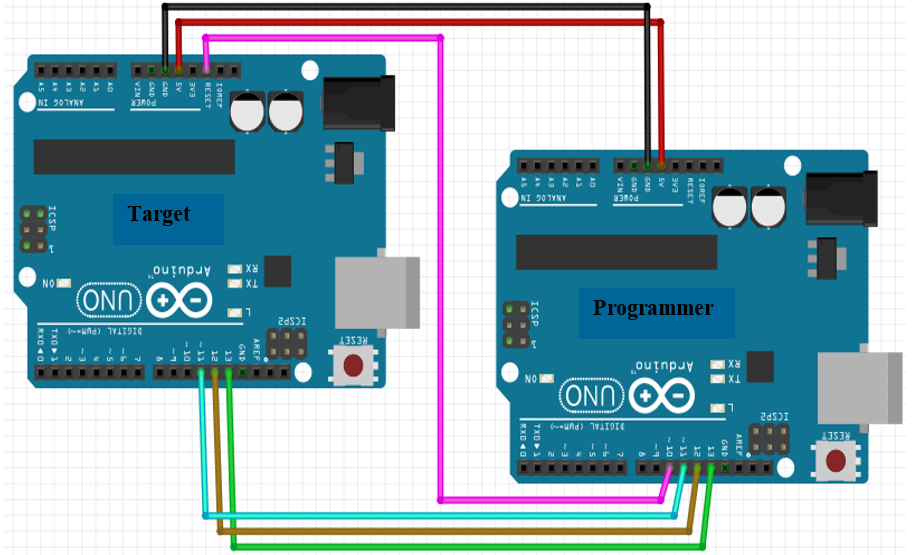
\includegraphics[scale=0.7]{EXP_04_Images/fig1.png}
\end{center}
\vspace{-7mm}
\begin{center} {Figure 1. Tool bar of Arduino IDE}\end{center}
\vspace{-3mm}
\begin{center} 
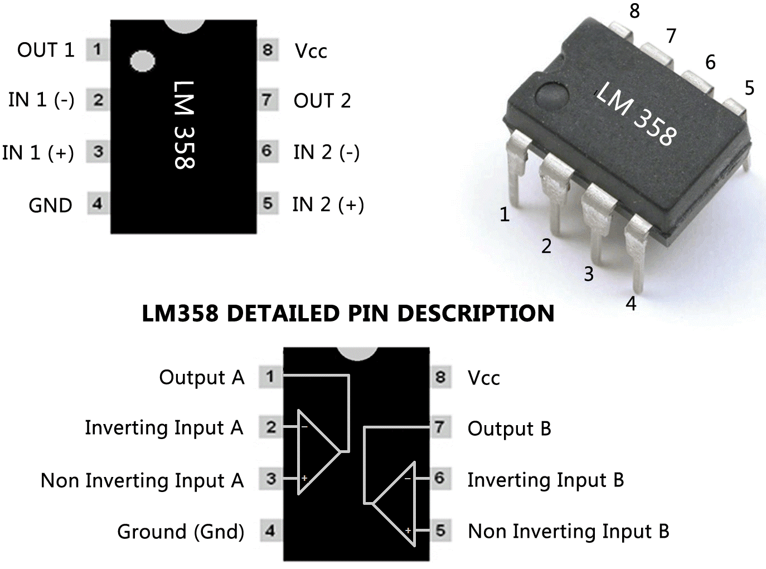
\includegraphics[scale=1]{EXP_04_Images/fig2.png}
\end{center}
\vspace{-7mm}
\begin{center} {Figure 2. Baud rate selection}\end{center}
\vspace{-3mm}
\noindent \textbf{Example 1:} We define a string array as \textbf{'my\_str[6]'} with six elements. We assign a character for each element of the string. Finally, we print it on the serial monitor. See the code below.
\end{justify}
\vspace{-5mm}
\hspace{1.5cm}\textbf{\large Code:}\\[6pt]
\setlength{\parindent}{8eM}

void setup() \{
   \textcolor{blue}{// set the speed for the serial monitor:}\\
 Serial.begin(9600);\\
 \textcolor{blue}{//set an array big enough for a five-character string:}\\
 char my\_str[6];\\    
  \textcolor{blue}{// the string consist of 5 characters:}\\
  my\_str[0] = 'H';  \\
  my\_str[1] = 'e';\\
  my\_str[2] = 'l';\\
  my\_str[3] = 'l';\\
  my\_str[4] = 'o';\\
  my\_str[5] = 0; \textcolor{blue}{ // 6th array element is a null terminator}\\
 \textcolor{blue}{// Print a String declared above using Serial.print() function}\\
  Serial.println(my\_str);\\
 \}\\
 void loop() \{\\
  \textcolor{blue}{// leave empty for now}\\
 \}\\

\setlength{\parindent}{0eM}
\begin{justify}
\noindent \textbf{Example 2:} We display the message on the serial monitor, take string input from the user, and print it. Initially, we define an integer variable 'count' with zero value stored in it. The number of characters of the string that is provided by the user is calculated, and the count variable is updated with this value and printed on the serial monitor alongwith other messages. See the code below.\end{justify}
\vspace{-5mm}
\hspace{1.5cm}\textbf{\large Code:}\\[6pt]
\setlength{\parindent}{8eM}

\textcolor{blue}{//Declare a string for incoming text}\\
String Name;\\
\textcolor{blue}{// Declare count as Integer and initializing it 0:} \\ 
int count = 0;\\[6pt]
void setup( )\\
\{\\
 \textcolor{blue}{// set the speed for the serial monitor:}\\
 Serial.begin(9600);\\
\textcolor{blue}{ // Print a String using Serial.print() function:}\\
 Serial.println("Hey! what's your name? ");\\
\}\\[6pt]
void loop( )\\
\{\\
  while ( Serial.available( ) )\\
  \{\\
  \textcolor{blue}{ // Print a String using Serial.print() function:}\\
   Serial.print("My name is: ");\\
  \textcolor{blue}{//Reading the Input string from Serial port:}\\
  Name = Serial.readString( );\\
  \textcolor{blue}{// Print a String using Serial.print() function:}\\
  Serial.println(Name);\\
  \textcolor{blue}{//Determine the length using .length():}\\
   int count = Name.length();\\
  \textcolor{blue}{//Print the length}\\
 Serial.print("It has");\\
 Serial.print(count);\\
 Serial.print(" characters in it.");\\
  \}\\
\}\\

\setlength{\parindent}{0eM}
\begin{justify}
\noindent \textbf{Example 3:} We have defined a string as a character array 'Name' having length 45 elements but have stored only 12 character string 'TalentSprint.' Observe the difference between function 'strlen()' and 'sizeof()' See the code below.\end{justify}
\vspace{-5mm}
\hspace{1.5cm}\textbf{\large Code:}\\[6pt]
\setlength{\parindent}{8eM}

void setup( ) \{\\
  \textcolor{blue}{// setting the baud rate for the serial monitor:}\\
  Serial.begin(9600);\\
 \textcolor{blue}{// Deceleration of a string and given the size of an array : }\\
 char Name[45] = "TalentSprint"; \\
 \textcolor{blue}{// Declare count as integer and initializing it 0: } 
  int  count = 0;\\
 \textcolor{blue}{// Print a String declared above using Serial.print() function:}\\
  Serial.print("Name = ");\\
  Serial.println(Name);\\
  \textcolor{blue}{// determine length using strlen() function and put the value in count}\\
  count = strlen(Name);\\
  Serial.print("Length of Name with strlen: ");\\
  Serial.println(count);\\
  \textcolor{blue}{// determine array size using sizeof() function and put the value in count}\\
  count = sizeof(Name);\\
  Serial.print("Length of Name with sizeof: ");\\
  Serial.println(count);\\
\}\\
void loop() \{\\
  \textcolor{blue}{// leave empty for now}\\
\}\\

\setlength{\parindent}{0eM}
\begin{justify}
\textbf{\underline{Math Libray}}\\
The Arduino Math library (math.h) has many useful mathematical functions for manipulating integer and floating-point numbers. The library has many macros defined also. A macro is defined as a piece of code in a program that is replaced by the macro value. Whenever the compiler encounters a macro name, it returns the name with the definition of the macro. Few commonly required math library macros are given in table 1 below.

\begin{center}{Table 1. Few useful macros}\end{center}
\vspace{-3mm}
\begin{center} 
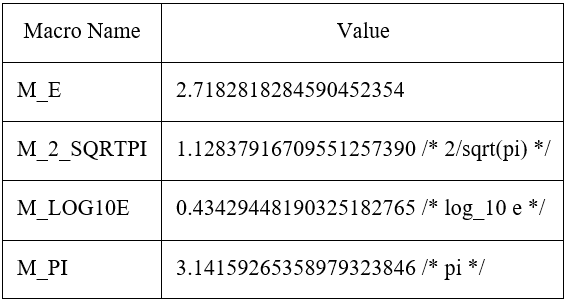
\includegraphics[scale=0.7]{EXP_04_Images/table1.png}
\end{center}

\noindent To include the libraries we use the \#include directive, for example \#include <math.h>. But for the latest Arduino IDE versions, the math library is included by default, so we don't require using the \#include directive.In the examples below, few functions of the math library will be used.\par 
\noindent \textbf{Example 1:} The user is asked to put the radius of the circle from the serial monitor. The area is calculated and printed on the serial monitor. The red LED glows for areas smaller than 100 units; for an area smaller than 1000 units, green LED glows, and any other calculated area, blue LED glows. Follow the code given below.\par
\noindent \textbf{Hardware/Software Setup:} Connect red, green, and blue LEDs to Pins 8, 9, 10, respectively. The software setup remains the same as in the previous example.
\end{justify}

\vspace{-5mm}
\hspace{1.5cm}\textbf{\large Code:}\\[6pt]
\setlength{\parindent}{8eM}

\#include $<$math.h$>$ \textcolor{blue}{// not required for latest ide versions}\\
int ledPin\_R = 8; \textcolor{blue}{// LED connected to digital pin 8}\\
int ledPin\_G = 9; \textcolor{blue}{// LED connected to digital pin 9}\\
int ledPin\_B = 10; \textcolor{blue}{// LED connected to digital pin 10}\\
double radius; \\
double area;\\
String msg = "Please enter the radius of the circle:" ;\\[9pt]
void setup() \{\\
  pinMode(ledPin\_R, OUTPUT); \textcolor{blue}{// sets the pin as output}\\
  pinMode(ledPin\_G, OUTPUT);\\
  pinMode(ledPin\_B, OUTPUT);\\
  Serial.begin(9600); \\
\}\\[9pt]
void loop() \{\\
  Serial.println(msg);\\
  radius = Serial.parseFloat( );  \textcolor{blue}{// It will read the incoming float}\\

  if (Serial.available( ) != 0) \{\\  
  
  Serial.print("The circle area for radius:");\\
  Serial.print(radius);\\
  Serial.print(" unit is : ");\\
  area=M\_PI*square(radius);\\
  Serial.println(area); \\   
  
  if (area$<$100) \{\\
    digitalWrite(ledPin\_R,HIGH);\\
    digitalWrite(ledPin\_G,LOW);\\
    digitalWrite(ledPin\_B,LOW);\\
  \}\\ 
  else if (area$<$1000) \{\\
    digitalWrite(ledPin\_R,LOW);\\
    digitalWrite(ledPin\_G,HIGH);\\
    digitalWrite(ledPin\_B,LOW);\\
  \}\\
  else \{\\
   digitalWrite(ledPin\_R,LOW);\\
    digitalWrite(ledPin\_G,LOW);\\
    digitalWrite(ledPin\_B,HIGH);\\
  \}\\
  \}\\
  delay(3000);\\
  \}

\setlength{\parindent}{0eM}
\begin{justify}
\noindent \textbf{Example 2:} We are going to plot a function and visualize it on the serial plotter. Consider the equation of current at time 't' is given by, i=1000*exp (-0.05*t)*sin (0.5*t). We are going to plot a nice curve showing how the current is changing with time. Note that the time variable t is in seconds, and millis() gives in milliseconds.\par
\noindent \textbf{Hardware/Software Setup:} Since we are just using an equation and plotting it on the serial plotter, we don't need any other hardware than Arduino board. Just connect it with a PC and upload the code. For visualizing the plot go to the 'Tools' and then select the 'Serial Plotter'. Similarly, for TinkerCAD, drag the Arduino board on the dashboard, dump the code, and simulate it.
\end{justify}
\vspace{-5mm}
\hspace{1.5cm}\textbf{\large Code:}\\[6pt]
\setlength{\parindent}{8eM}

  double i;\\
  double t;\\
  void setup() \{\\
  Serial.begin(9600); \}\\
  void loop() \{\\
  t=millis()/1000;\\
  i=1000*exp(-0.05*t)*sin(0.5*t);\\
  Serial.println(i);\\
  delay(1000);\\
  \}\\[9pt]

The plot on Serial Plotter looks like as given below.
\vspace{-4mm}
\begin{center} 
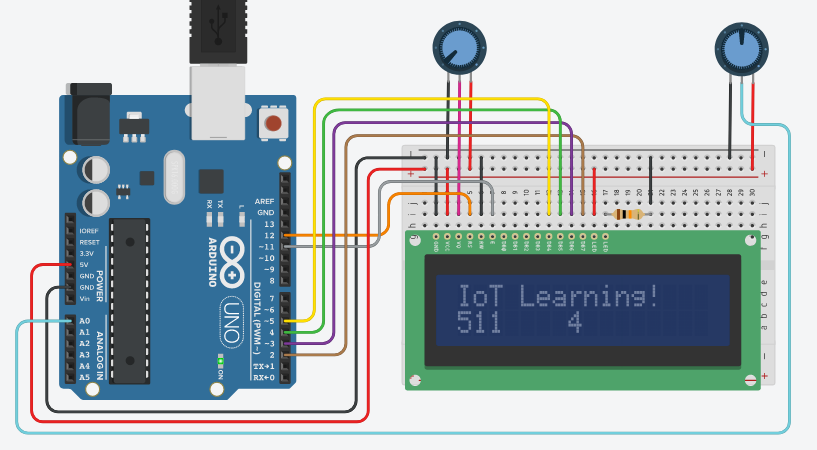
\includegraphics[scale=0.8]{EXP_04_Images/fig3.png}
\end{center}
\vspace{-7mm}
\begin{center} {Figure 3. Plot on serial plotter}\end{center}
\vspace{-3mm}

\setlength{\parindent}{0eM}
\begin{justify}
\textbf{\underline{Digital Read Function}}\\
We have already used the 'digitalWrite()' function in the 'LED blinking with Arduino' experiment. Following is the syntax and parameter for 'digitalRead()' function. The function reads the value from the specified digital pin, either HIGH or LOW.

\noindent \textbf{Syntax }- digitalRead(pin)\\
\textbf{Parameters }- pin: the Arduino PIN you want to read

\noindent\textbf{Example:} We will implement the digitalRead() function, and Pin 7 is used as digital read Pin. Pin 7 gets triggered as HIGH when the push button is pushed since the circuit from 5V and GND gets connected through the resistor and LED connected to Pin 13 glows. Code for the example given below.\par
\noindent \textbf{Hardware/Software Setup :} We can connect the hardware the same as in the TinkerCAD diagram below. The software setup remains the same as in the previous example
\end{justify}

\vspace{-4mm}
\begin{center} 
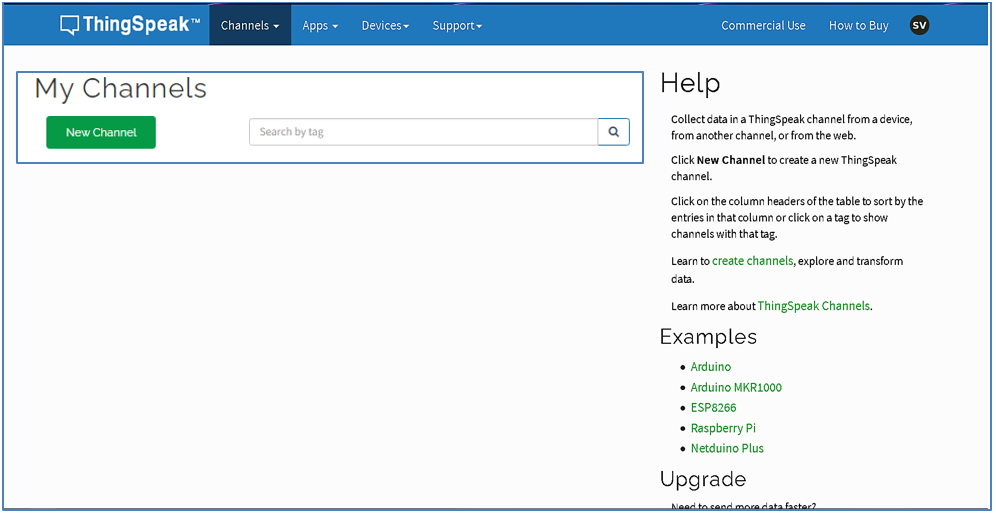
\includegraphics[scale=0.9]{EXP_04_Images/fig4.png}
\end{center}
\vspace{-7mm}
\begin{center} {Figure 4. Hardware setup for demonstration of digital read function}\end{center}
\vspace{-3mm}

\hspace{1.5cm}\textbf{\large Code:}\\[6pt]
\setlength{\parindent}{8eM}

int led\_Pin= 13;  \textcolor{blue}{// LED connected to digital pin 13}\\
int input\_Pin = 7; \textcolor{blue}{  // pushbutton that is connected to the digital pin 7}\\
int val = 0; \textcolor{blue}{  // declaring the variable to store the read value}\\
void setup() \{\\
  pinMode(led\_Pin, OUTPUT);\textcolor{blue}{  // sets the digital pin 13 as output}\\
  pinMode(input\_Pin, INPUT); \textcolor{blue}{   // sets the digital pin 7 as input}\\
\}\\
void loop() \{\\
  val = digitalRead(input\_Pin); \textcolor{blue}{ // read the input pin}\\
    digitalWrite(led\_Pin, val);\\
\}\\

\setlength{\parindent}{0eM}
\begin{justify}
\textbf{\underline{Analog Read and Analog Write Function}}\\[3pt]
\textbf{analogRead()}\\[6pt]
\noindent The function reads the value from the specified analog pin. The Arduino boards contain a multichannel, 10-bit analog to digital converter. This means the functions will map the input voltages between 0 and the operating voltage of MCU (5V or 3.3V) into the integer values between 0 and 1023. For example, an Arduino UNO yields a resolution between the readings of 5 volts / 1024 units or 0.0049 volts (4.9 mV) per unit.\par
\noindent \textbf{Syntax }- analogRead(pin)\\[3pt]
\textbf{Parameters }- pin: the name of the analog input pin to read from (A0 to A5 on most boards)\\[3pt]
\textbf{Returns} - The analog reading on the pin. However, it is limited to the resolution of the analog to digital converter (0-1023 for 10 bits or 0-4095 for 12 bits). Data type: int.\par
\noindent \textbf{analogWrite()}\\[3pt]
The function writes an analog value (PWM wave) to the specified pin. It can also be used to light an LED at varying brightnesses or drive a motor at required speeds. After a call to the analogWrite(), the pin will generate a steady rectangular wave of specified duty cycle until the next call to the analogWrite() (or a call to the digitalRead() or digitalWrite()) on the same pin.\par
\noindent \textbf{Syntax} - analogWrite(pin, value)\\[3pt]
\textbf{Parameters} - pin: the Arduino pin to write. Allowed data types are int value: the duty cycle: between 0 (always off) and 255 (always on). Allowed data types are int.\par
\noindent \textbf{Example: } We are going to implement both analogRead() and analogWrite() function. Inputs(outer Pins) of the Potentiometer are connected to 5V and GND, and the output(middle pin) is connected to the analog read Pin A4. LED is connected to Pin 10, which is used as an analog write pin. Value of analog read increase or decrease based on the position of Potentiometer and corresponding analog write operation is done on the LED pin. Thus we can observe the changing brightness of the LED.\par
\noindent \textbf{Hardware/Software Setup: } We can connect the hardware the same as in the TinkerCAD diagram below. The software setup remains the same as in the previous example.
\end{justify}
\vspace{-4mm}
\begin{center} 
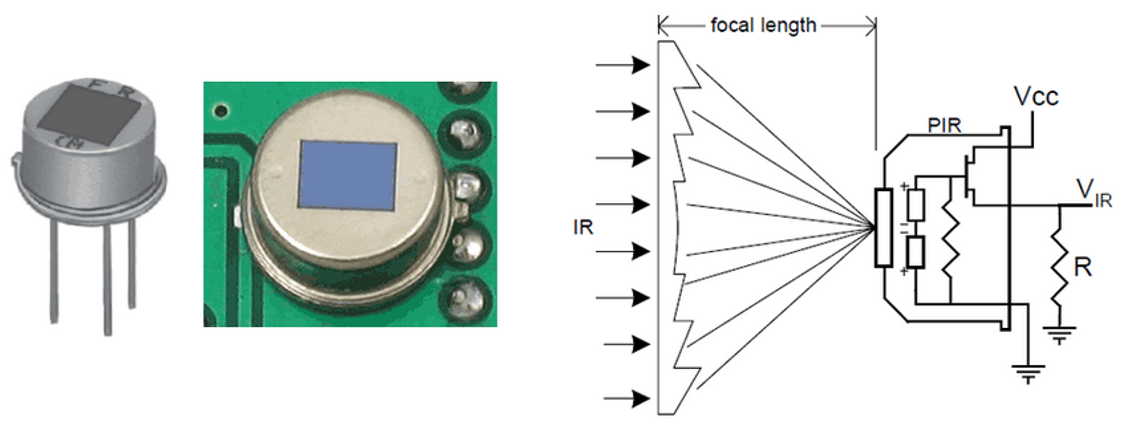
\includegraphics[scale=0.9]{EXP_04_Images/fig5.png}
\end{center}
\vspace{-7mm}
\begin{center} {Figure 5. Hardware setup for demonstration of anlog read/write function}\end{center}
\vspace{-3mm}



\hspace{1.5cm}\textbf{\large Code:}\\[6pt]
\setlength{\parindent}{8eM}

int led\_Pin = 10; \textcolor{blue}{  // LED connected to digital pin 10}\\
int analog\_Pin = 4; \textcolor{blue}{  // potentiometer connected to analog pin 4}\\
int val = 0; \textcolor{blue}{ // declaring variable to store the read value}\\[9pt]
void setup() \{\\
  pinMode(led\_Pin, OUTPUT); \textcolor{blue}{ // sets the pin as output}\\
\}\\[9pt]
void loop() \{\\
  val = analogRead(analog\_Pin); \textcolor{blue}{ // read the input pin}\\
  analogWrite(led\_Pin, val/4); \textcolor{blue}{// analogRead values go from 0 to 1023,\\ analogWrite values from 0 to 255}\\
\}

\setlength{\parindent}{0eM}
\begin{justify}
\textbf{\underline{Switch Cases}}\\[3pt]
We have already used the if-else statement, which allows us to choose between two discrete options, TRUE or FALSE. For more than two options, we can use multiple if statements. But for such situations, the switch statement is more suitable. A switch allows us to choose between several discrete options.\end{justify}


\hspace{1.5cm}\textbf{\large Syntax:}\\[6pt]
\setlength{\parindent}{8eM}

switch (var) \{\\
  case label1:\\
    \textcolor{blue}{// Some statements}\\
    break;\\
  case label2:\\
    \textcolor{blue}{// Some statements}\\
    break;\\
  default:\\
    \textcolor{blue}{// Some statements}\\
    break;\\
\}\\[6pt]
\textbf{Parameters:}\\[3pt] 
var: the variable whose value to compare with various cases.\\ Allowed data types are int, char.\\
label1, label2: constants. Allowed data types are int, char.


\setlength{\parindent}{0eM}
\begin{justify}
\textbf{Example: }We will use the 'Switch Cases' to turn on one of the several different LEDs based on the byte of data received serially. The sketch listens for the serial input and turns on a red, green, and blue LED for r, g, and b, respectively.\par
\noindent We have shown only three cases with 3 LEDs, but we can use as many cases as required based on the number of LEDs (task) we want. See the code below and note: how the three Pins 8, 9, and 10 are defined as output Pin mode using For loop.\par
\noindent \textbf{Hardware/Software Setup:} Connect red, green, and blue LEDs to Pins 8, 9, 10, respectively. The software setup remains the same as in the previous example.  \end{justify}

\vspace{-3mm}

\hspace{1.5cm}\textbf{\large Code:}\\[6pt]
\setlength{\parindent}{8eM}

void setup() \{\\
 Serial.begin(9600); \textcolor{blue}{ // initialize serial communication}\\
 for (int thisPin = 8; thisPin $<$ 11; thisPin++) \{    \textcolor{blue}{ // initialize the LED pins}\\
 pinMode(thisPin, OUTPUT);\\
 \}\\
 Serial.println("Pass r,g, or b for switching on \\red, green or blue LED          respectively.");\\
 \}\\[9pt]
void loop() \{\\
  if (Serial.available()$ > $0) \{\\
    int color=Serial.read();\\
     \textcolor{blue}{
    // do something depending on the character received.\\
    // switch statement expects a single number values for each case; in this\\
    // example, though, we're using single quotes to tell the controller to get\\
    // the ASCII value for the character. For example 'a' = 97, 'b' = 98,\\
    // and so forth:}\\
    switch (color) \{\\
      case 'r':\\
       digitalWrite(8, HIGH);\\
       digitalWrite(9,LOW);\\
       digitalWrite(10,LOW);\\
        break;\\
      case 'g':\\
        digitalWrite(9, HIGH);\\
        digitalWrite(8,LOW);\\
        digitalWrite(10,LOW);\\
        break;\\
       case 'b':\\
        digitalWrite(10, HIGH);\\
        digitalWrite(8,LOW);\\
        digitalWrite(9,LOW);\\
        break;\\
    \}\\
  \}\\
\}\\



\setlength{\parindent}{0eM}
\begin{justify}
\textbf{\underline{Defining and Calling a Function}}\\[6pt]
\textbf{Example:} We are going to define a function and call it inside another function. A function named 'get\_volts' is defined, converting the analog read value into equivalent voltage based on maximum ADC count and the reference voltage.\par

\noindent Inputs (outer Pins) of the Potentiometer are connected to 5V and GND, and the output (middle pin) is connected to the analog read Pin A2. LED is connected to Pin 13, which is used for the digital write. The value of analog read increases or decreases based on the position of the Potentiometer and is stored in a variable named 'analogValue', which is also printed in the serial monitor. The calculated voltage from the 'get\_volts' is printed on the serial monitor and compared with a threshold value. Pin 13 gets HIGH as a digital write command, and LED glows if the computed voltage exceeds the threshold value.\par

\noindent \textbf{Hardware/Software Setup:} We can connect the hardware the same as in the TinkerCAD diagram below. The software setup remains the same as in the previous example.

\begin{center} 
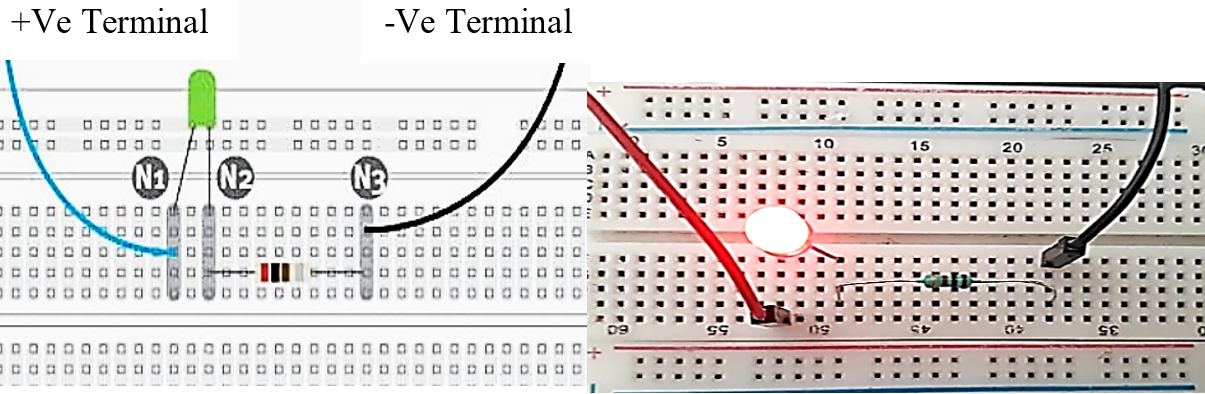
\includegraphics[scale=0.9]{EXP_04_Images/fig6.png}
\end{center}
\vspace{-7mm}
\begin{center} {Figure 6. Hardware setup for demonstration of defining/calling a function}\end{center}
\end{justify}


\vspace{10mm}
\hspace{1.5cm}\textbf{\large Code:}\\[6pt]
\setlength{\parindent}{8eM}


const int analogPin = A2; \textcolor{blue}{ //Pin that potentiometer output is attached to}\\
const int ledPin = 13;  \textcolor{blue}{ // Pin that the LED is attached to}\\
const float threshold = 2.5;  \textcolor{blue}{  // an arbitrary threshold level that's in the \\range of the analog input}\\
 \textcolor{blue}{//Defining a function}\\[9pt]
float get\_volts(int raw\_input, int max\_adc\_count,  float ref\_volt)\{\\
    float volts = 0.0;\\
    volts = (raw\_input*ref\_volt)/max\_adc\_count; \\ \textcolor{blue}{ // calculate actual voltage}\\
return volts;\\
\}\\[9pt]
void setup() \{\\
  pinMode(ledPin, OUTPUT);  \textcolor{blue}{// initialize the LED pin as an output:}\\
  Serial.begin(9600);\\
\}\\[9pt]
void loop() \{\\
   \textcolor{blue}{// read the value of the potentiometer:}\\
  int analogValue = analogRead(analogPin); \\
  Serial.println(analogValue);\\
  float volts = get\_volts(analogValue, 1023, 5.0); \\
  Serial.println(volts); \\
   \textcolor{blue}{//  if the analog value is high enough then turn on the LED:}\\
  if (volts$ > $threshold) \{\\
    digitalWrite(ledPin, HIGH);\\
  \} \\
  else \{\\
    digitalWrite(ledPin, LOW);\\
  \}\\  
  delay(2000);  \textcolor{blue}{// the delay in between reads for stability}\\
\}\\

\vspace{10cm}

\setlength{\parindent}{0eM}
\begin{justify}
\noindent \textbf{\large REFERENCES:}
\vspace{-3mm}
\begin{enumerate}
 \setlength\itemsep{-0.3em}
 
\item \href{https://www.arduino.cc/reference/en/language/functions/communication/serial/write/}{Serial Write}

\item \href{https://www.arduino.cc/reference/en/language/functions/communication/serial/read}{Serial Read}

\item \href{https://www.arduino.cc/reference/en/language/variables/data-types/string/}{String}

\item \href{https://www.arduino.cc/en/math/h}{Math}

\item \href{https://www.arduino.cc/reference/en/language/functions/digital-io/digitalread}{Digitalread }


\item \href{https://www.arduino.cc/reference/en/language/functions/analog-io/analogread/}{Analogread }

\item \href{https://www.arduino.cc/reference/en/language/functions/analog-io/analogwrite/}{Analogwrite}

\item \href{https://www.arduino.cc/en/Tutorial/BuiltInExamples/ifStatementConditional}{If Statement \& Conditional }


\item \href{https:/www.arduino.cc/en/Tutorial/BuiltInExamples/ForLoopIteration}{Foor Loop}

\item \href{https://docs.arduino.cc/built-in-examples/control-structures/SwitchCase2}{SwitchCase}

\end{enumerate}

\noindent \textbf{\large CONCEPT DRILLS:}
\vspace{-3mm}
\begin{enumerate}
 \setlength\itemsep{-0.3em}
\item  Mimic a simple traffic signal control system using Red, Green, and Blue LEDs. Initially, all the LEDs are turned off. The LEDs are turned on one at a time with a delay of 5 seconds . When Green LED glows, the 'GO' message should be displayed on the serial monitor. Similarly for Red and Blue LEDs, the message should be 'STOP' and 'WAIT' respectively.
\item  Design a circuit with an LED, two pushbuttons, and a buzzer with appropriate code so that buzzer starts making a sound, and the LED also glows when the first push button is triggered. Only LED glows when the second Push button is triggered. Hints: Use digitalRead() and related concept.
\item  Design a circuit with three different colored LEDs and a potentiometer with appropriate code. The LEDs should turn on one by one as we rotate the potentiometer. Hints: Use anlogRead()/Write() and related concept.
\end{enumerate}
\vspace{10cm}

\begin{center} \textbf{\large APPENDIX} \end{center}

\noindent \textbf{\underline{Serial Communication}}\\[6pt]
Serial communication is a scheme that uses the Universal Asynchronous Receiver/Transmitter (UART) on the Microcontroller. The messages are sent in the form of 8 bits or 1 byte, where 1 byte = 8 bits.
The Arduino sent the messages to the computer/other devices from Pin 1of the board, called Tx (Transmitter), and receives the messages from the computer on Pin 0, called Rx (Receiver).
Once we initialize these Pins for serial communication in our code, these can't be used for any other use case. The pins Tx and Rx are connected to the computer directly. These are connected to the Tx and Rx serial chip and behave as the serial to USB translator. This acts as the medium for the computer to talk to the Microcontroller. 
Followings are the few frequently used functions of the Serial class available in Arduino for communicating with computer/other devices.\\[6pt]
\textbf{Serial.begin (speed):} The function tells the serial object to initialize as to receive and send data on the Rx and Tx, which are pins 1 and 0. Here 'speed' sets the baud rate for serial data communication. The baud rate signifies the data rate in bits per second.\\[6pt]
\textbf{Serial.print():} It prints the data to the serial port.\\[6pt]
\textbf{Serial.println():} It prints the data followed by the carriage return ('\textbackslash r' or ASCII 13) and newline ('\textbackslash n' or ASCII 10) characters. \\[6pt]
\textbf{Serial.available():} This function in Arduino gets the stored bytes from the serial port that are available for reading. It is the data, which is already stored and arrived in the serial buffer. The serial buffer in Arduino holds 64 bytes.\\[6pt]
\textbf{Serial.read():} The function reads the incoming data in the Arduino. The data type int is used here. The function returns the first data byte of the arriving data. It returns -1 when no data is available on the serial port.\\[6pt]
\textbf{Serial.readString():} The function reads the incoming serial data from the serial buffer in the string. \\[6pt]
\textbf{Serial.parseFloat():} It returns the first valid floating-point number from the Serial buffer. It is terminated by the first character that is not a floating-point number. The function terminates if it times out.\\[6pt]
\textbf{Serial.parseInt():} It returns the first valid integer number from the Serial buffer. parseInt() function is terminated by the first character if it is not an integer number. The function terminates if it times out.\\[6pt]
\textbf{Serial.write():} The function sends the binary data to the serial port of the Arduino. The data through the function is sent as a series of bytes or a single byte. And if we want to send the digits of numbers represented by the characters, we need to use the Serial.print ( ) function instead of Serial.write ().



\end{justify}
\end{document}